\documentclass{beamer}
\usetheme{Berlin}
\usecolortheme{dolphin}

\usepackage[T1]{polski}
\usepackage[polish]{babel}
\usepackage[utf8]{inputenc}
\usepackage[T1]{fontenc}
\usepackage[mediumspace,mediumqspace,Grey,squaren]{SIunits}
\usepackage{graphicx}
\usepackage{hyperref}

%\addbibresource{bibliography.bib}

%\setbeamertemplate{bibliography item}{\insertbiblabel}


\graphicspath{ {./images/} }

\begin{document}
\title{Seminarium dyplomowe magisterskie}
\author{Jakub Postępski}
\date{29 listopada 2018}

\frame{\titlepage}

\section{Zarys pracy magisterskiej}
\begin{frame}{Sterowanie ramieniem robota w obliczu chwytania przedmiotów}

\begin{itemize}
\item Dr inż. Tomasz Winiarski
\end{itemize}

\begin{itemize}
\item Sterowanie siłowe
\item Odczyty wartości z efektorów i receptorów
\item Nieznany model chwytanego obiektu
\end{itemize}
\end{frame}


\begin{frame}{Robot usługowy Velma}
\begin{itemize}
\item Dwa manipulatory LWR (sterowanie impedancyjne)
\item Chwytaki Barretta (sztuczna skóra, czujniki siły)
\item Nadgarstkowe czujniki siły i momentu 
\item Kinect
\item Stereopara
\item Komputer sterujący
\end{itemize}
\end{frame}

\begin{frame}{Zdjęcie robota Velma}
\begin{figure}[h]
	\centering
	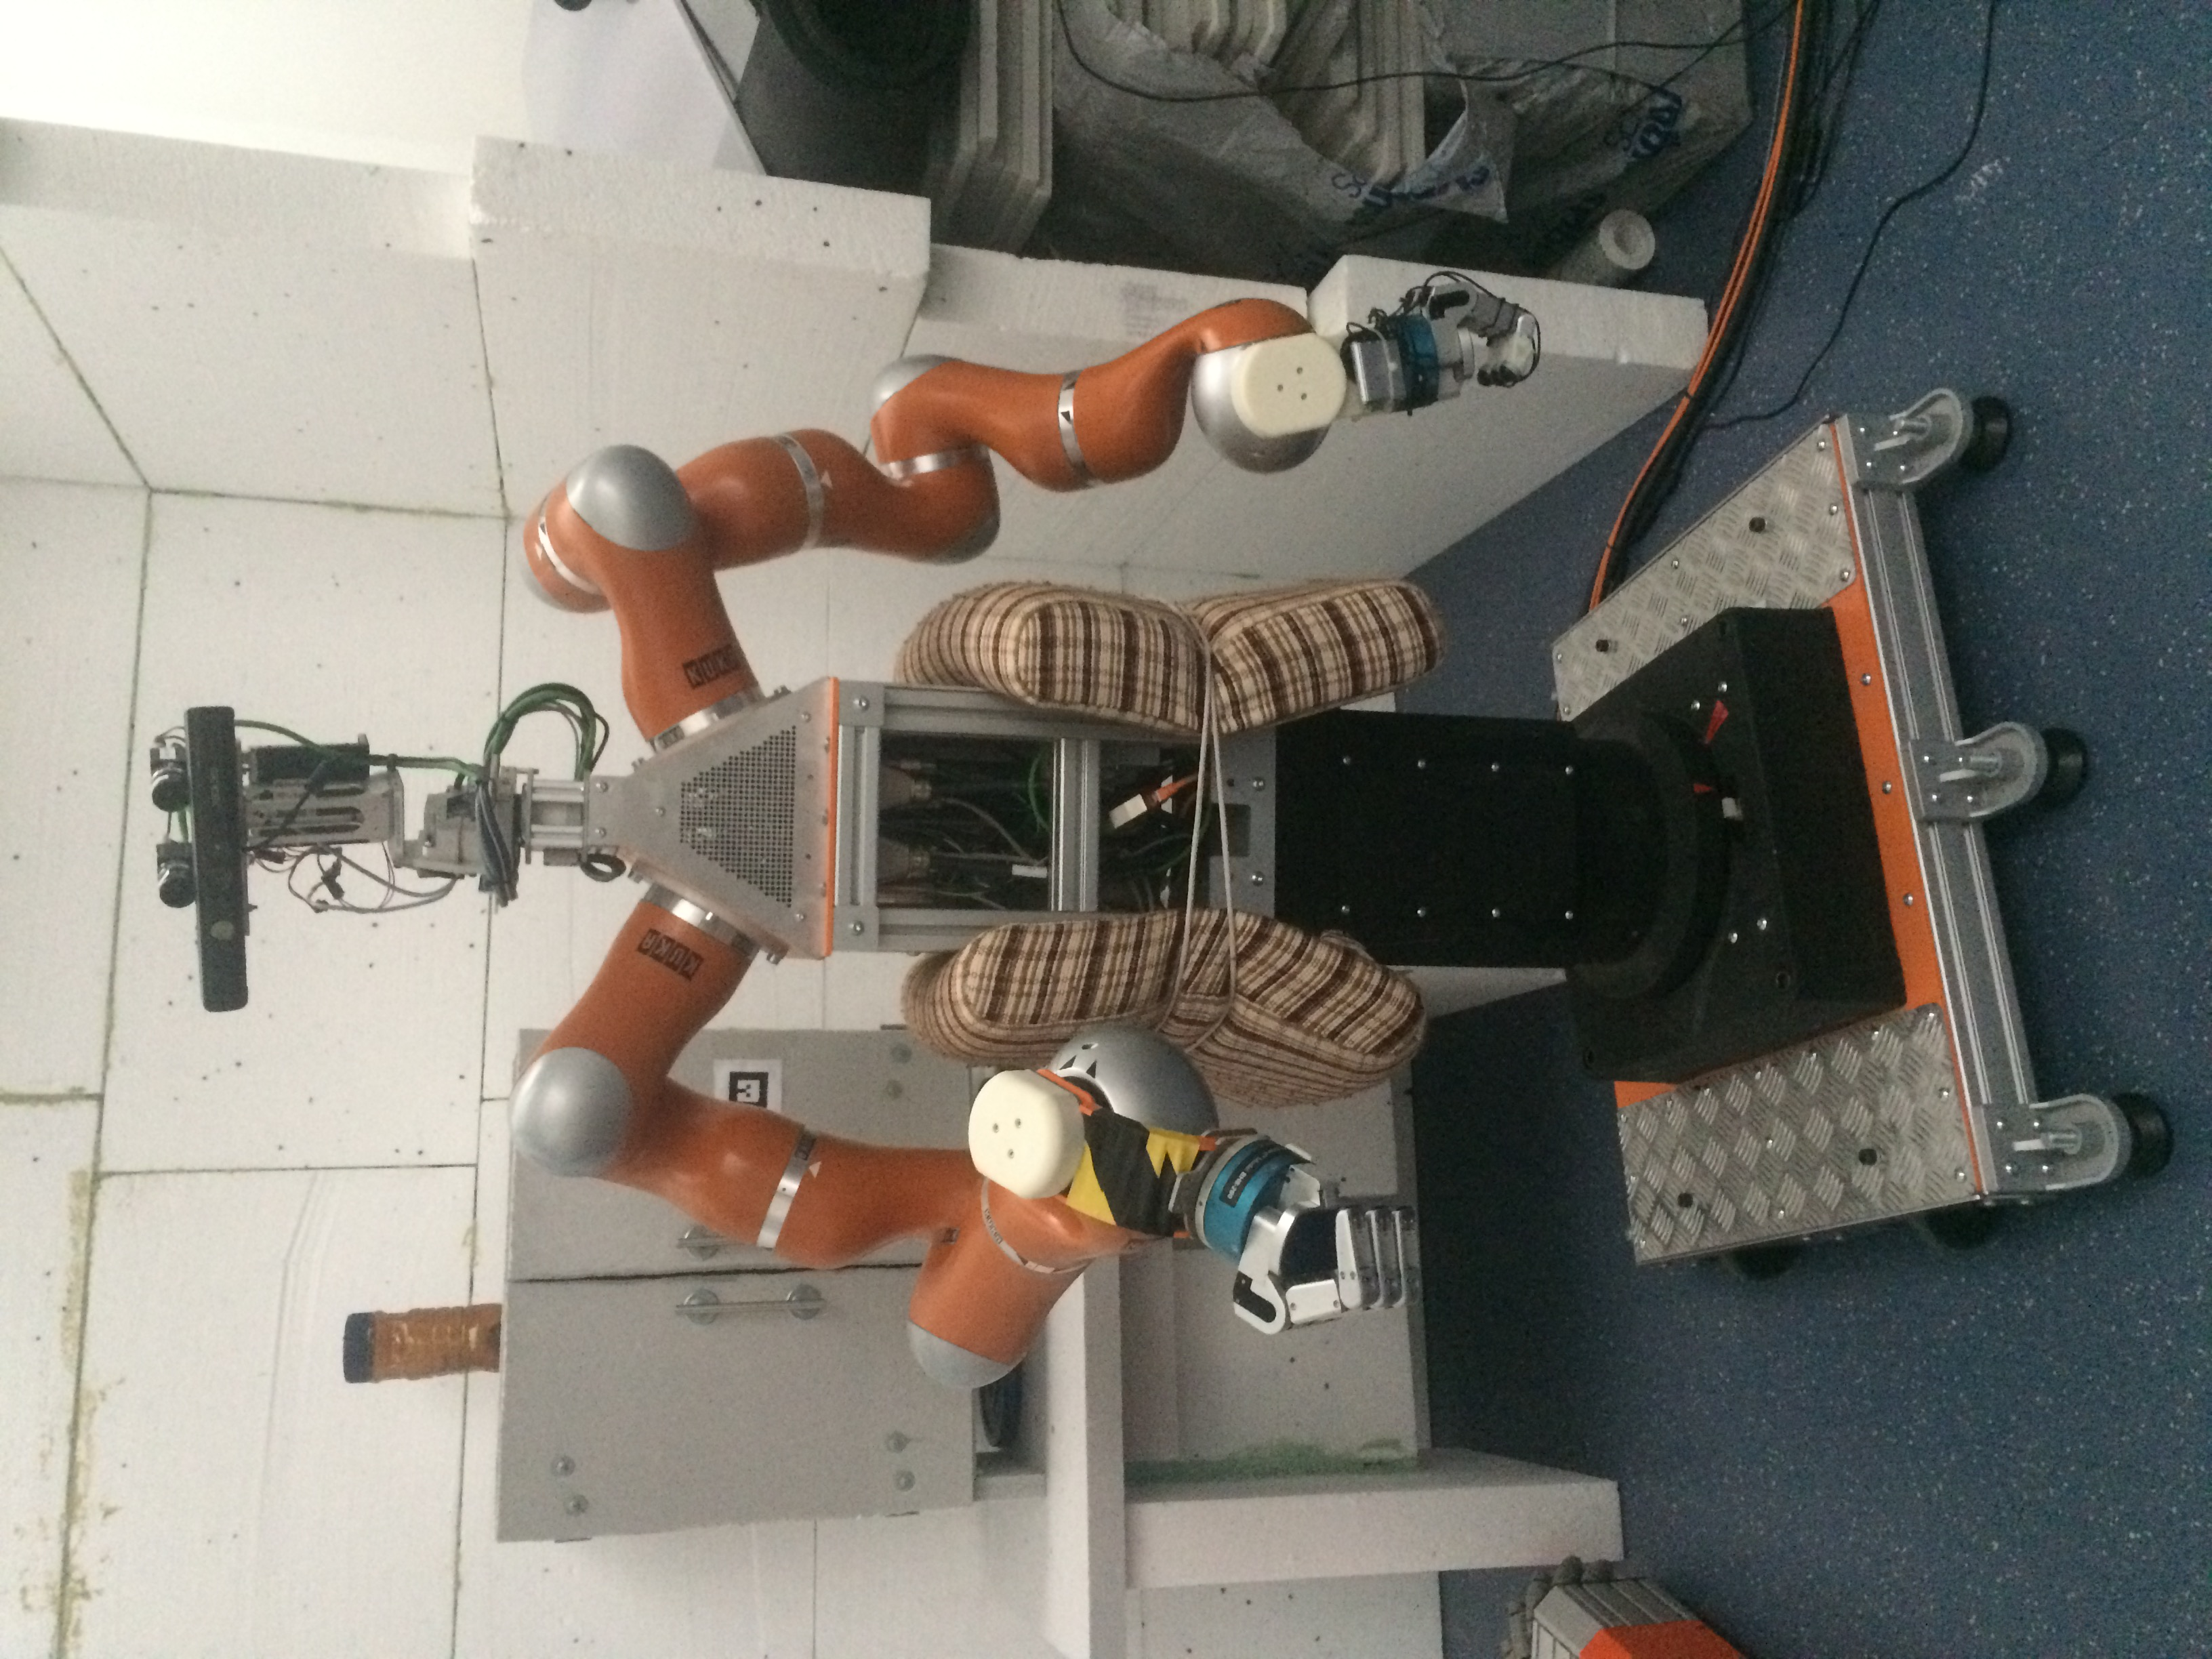
\includegraphics[scale=0.06, angle =-90]{velma1}
\end{figure}

\end{frame}

\begin{frame}{Struktura oprogramowania}

Struktura komponentowa. Częstotliwość pętli sterowania to 500 Hz.

\begin{itemize}
	\item ROS
	\item Orocos
\end{itemize}

Symulator działania z modelem fizyki i symulacją czasu.


\begin{itemize}
	\item Gazebo
	\item Dart
\end{itemize}
\end{frame}

\section{Koncepcja rozwiązania problemu}
\begin{frame}{Przestrzenie operacyjne}
\begin{itemize}
	\item Stawów
	\item Operacyjna
\end{itemize}

Do transformacji współrzędnych służy Jakobian.
\end{frame}

\begin{frame}{Sterowanie impedancyjne}
	\begin{figure}[h]
		\centering
		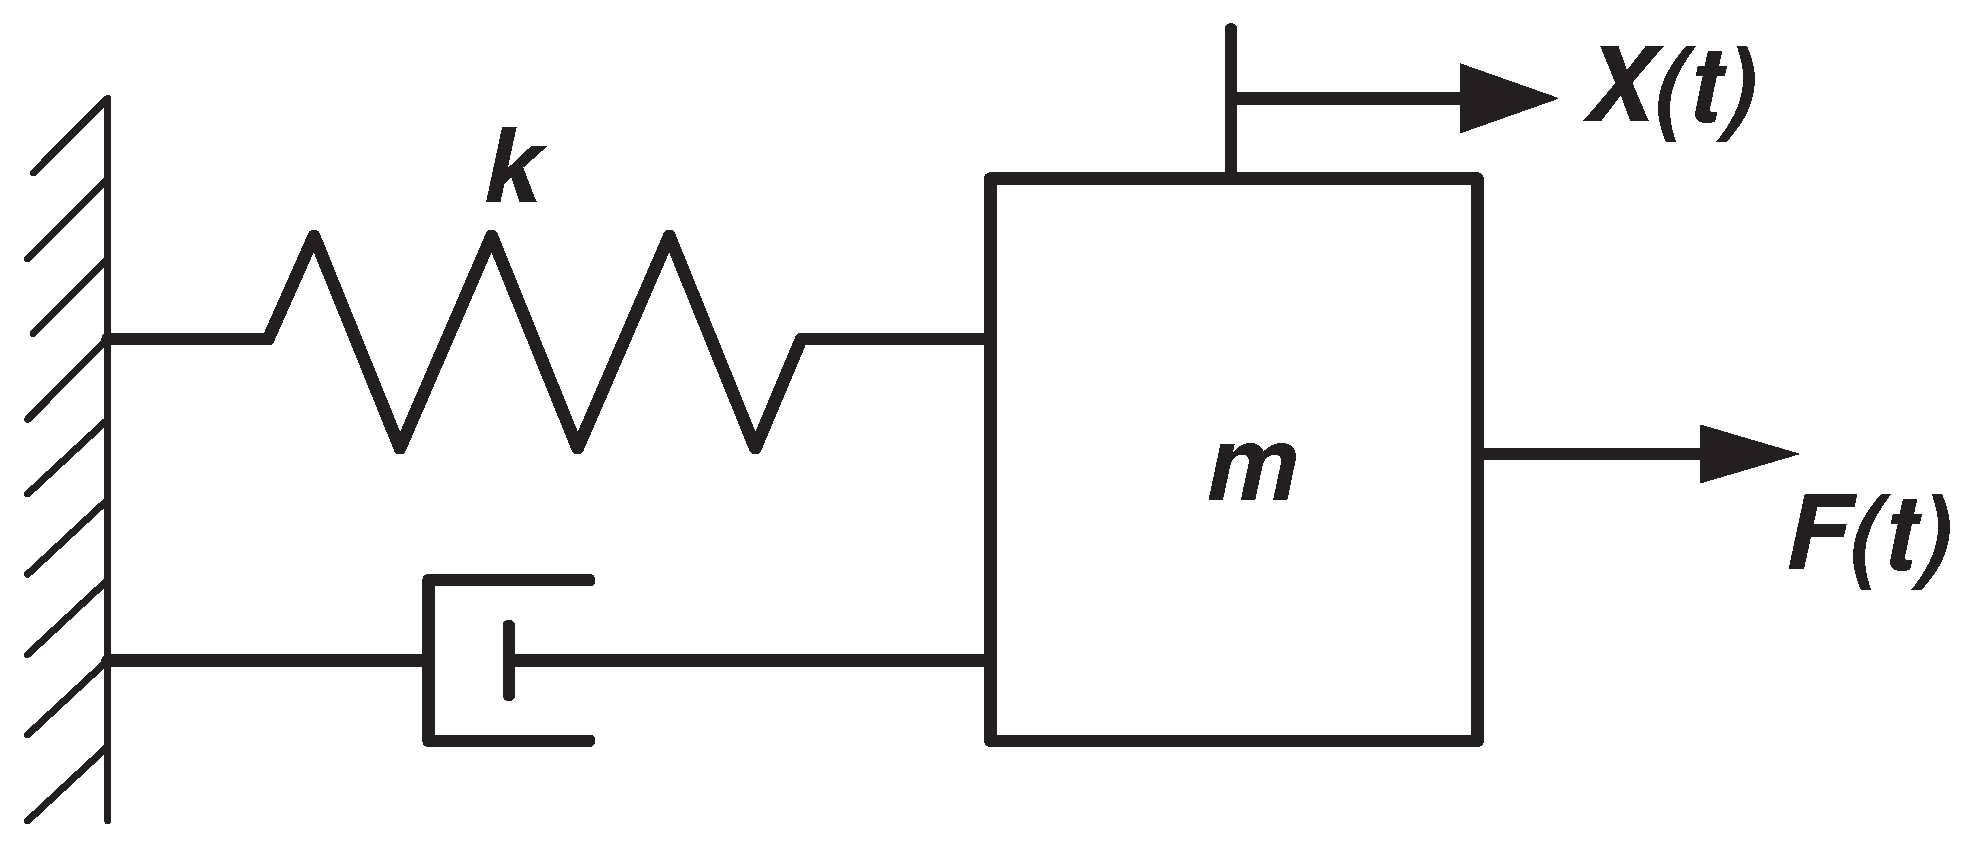
\includegraphics[scale=1.30]{mds}
	\end{figure}

\begin{equation}
F = kx + d\dot{x} + F_{ext}
\end{equation}
\end{frame}

\begin{frame}{Model robota}
Dla członu i-tego mamy:
\begin{itemize}
	\item Masa $m_i$
	\item Tensor bezwładności $I_{3x3}$ (macierz semisymetryczna)
	\item Macierz inercji $M_{xi 6x6}$
\end{itemize}
\begin{equation}
M_{xi}=
\begin{bmatrix}
m_i & 0 & 0 & 0 & 0 & 0 \\
0 & m_i & 0 & 0 & 0 & 0 \\
0 & 0 & m_i & 0 & 0 & 0 \\
0 & 0 & 0 & I_{xx} & I_{xy} & I_{xz} \\
0 & 0 & 0 & I_{yx} & I_{yy} & I_{yz} \\
0 & 0 & 0 & I_{zx} & I_{zy} & I_{zz} \\

\end{bmatrix}
\end{equation}

Wniosek: Model chwytanego przedmiotu możemy opisać w ten sam sposób.
\end{frame}

\begin{frame}{Jak przeprowadzić symulację?}
\begin{equation}
\tau = K(q_d-q) + D(\dot{q}) + \hat{M}(q)\ddot{q_d} + \hat{c}(q, \dot{q}) + \hat{g}(q) + \hat{h}(q, \dot{q})
\end{equation}

\begin{equation}
	\dot{x} = J(q)\dot{q}
\end{equation}


\begin{equation}
\tau = M(q)\dot{\omega} + \omega \times M(q)\omega
\end{equation}

\begin{equation}
M(q) = \sum_{i=0}^{n}J_i^T(q)M_{xi}(q)J_i(q)
\end{equation}
\end{frame}


\begin{frame}{Estymacja parametrów}

Można zastosować optymalizację minimalizującą sumę błędów kolejnych odczytów:
\begin{equation}
e_t = \begin{bmatrix}
F_t - \hat{F_t}\\
\tau_t - \hat{\tau_t} 
\end{bmatrix}
\end{equation}

\begin{equation}
\begin{aligned}
& \underset{m, M(q)}{\text{min}}
& & \sum_{t = 1}^{T} || e_t ||
\end{aligned}
\end{equation}

\end{frame}

\section{Eksperymenty}
\begin{frame}{Symulowany układ}
\begin{figure}[h]
	\centering
	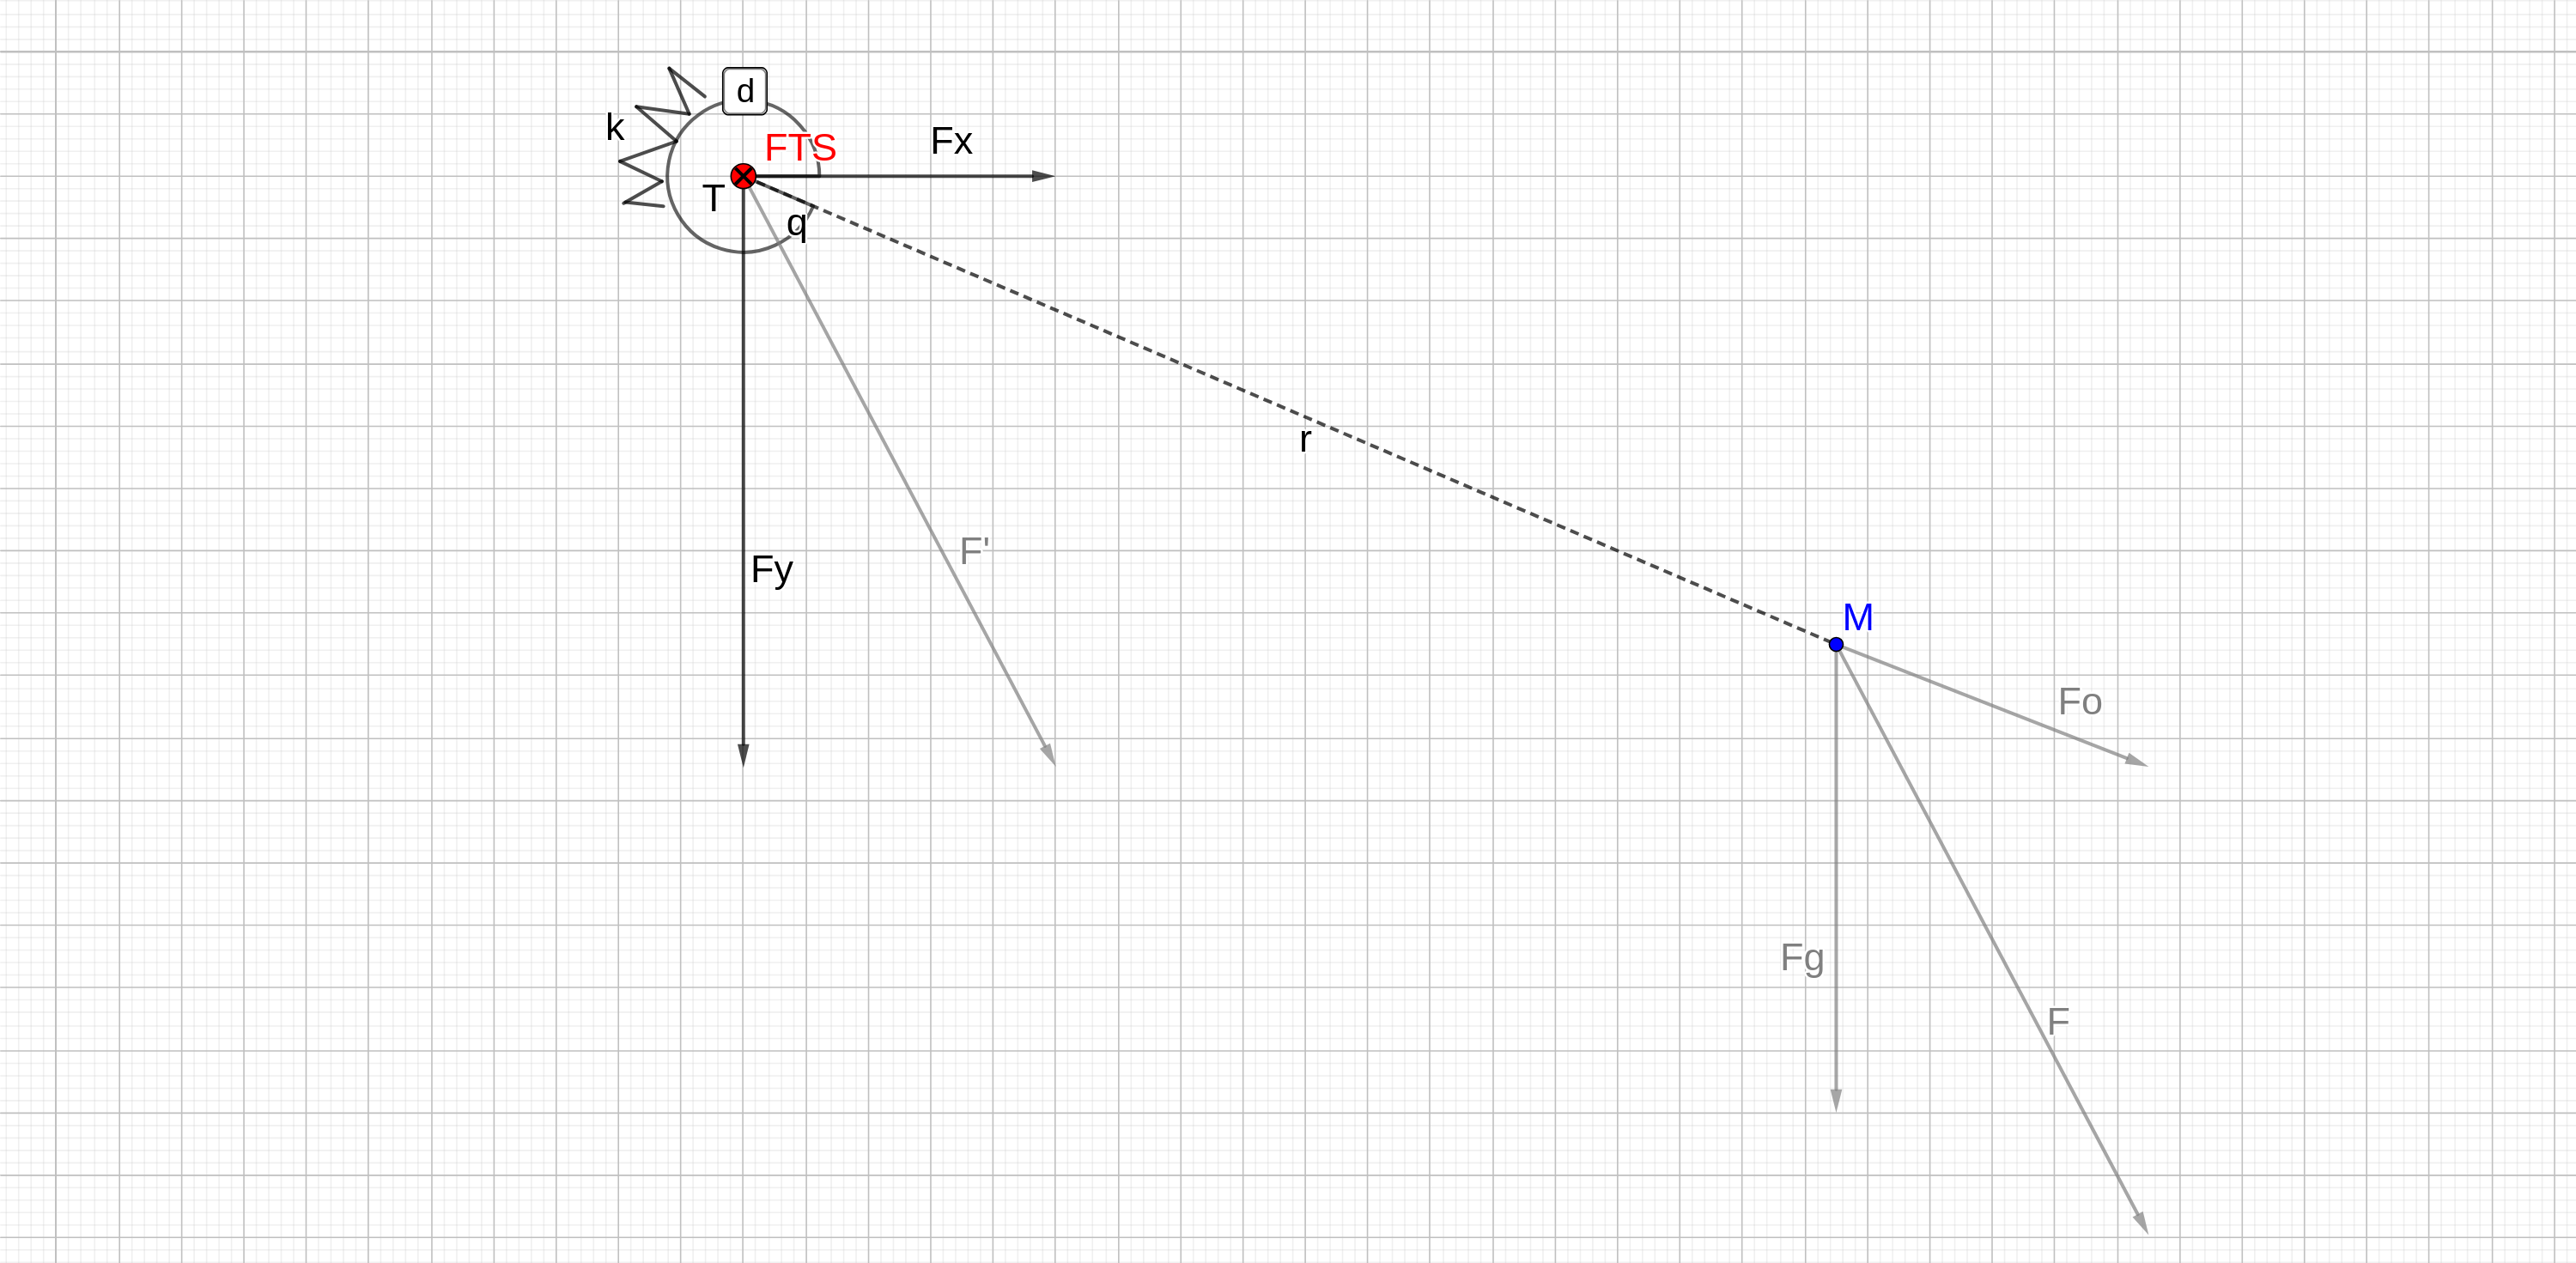
\includegraphics[scale=1.30]{2d}
\end{figure}


\end{frame}


%\begin{frame}[allowframebreaks]{Bibliografia}
%\bibliographystyle{plain}
%\bibliography{bibliography}
%\end{frame}
\section{Podsumowanie}
\begin{frame}{Bibliografia}
\begin{itemize}
	\item https://studywolf.wordpress.com/2013/09/07/robot-control-3-accounting-for-mass-and-gravity/
	\item Zdjęcia pochodzą ze strony \url{https://robotyka.ia.pw.edu.pl}
	 
\end{itemize}

\end{frame}
\begin{frame}{Dziękuję za uwagę}
\begin{figure}[h]
	\centering
	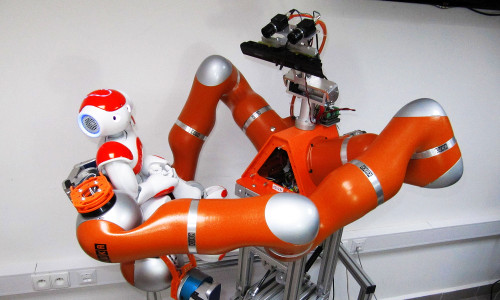
\includegraphics[scale=1.4]{velma3}
\end{figure}
\end{frame}
\end{document}